\section{Experimental Evaluation}
\label{exp}
%%%%%%%%%%% 1st experiment %%%%%%%%%%%%
% {\color {red} We evaluate the ....using two sets pf experiments: ...The first exdpriment what why.... the second what why? } WHAT
% WHY?
% HOW? 
% experimenta setup
% -dateset
% - environment
% Results and discussion 

We evaluate the proposed method using two sets of experiments. The objective of the first preliminary experiment is to demonstrate how the distributional properties in input data can impact the model performance. 
%Since real-world data distributions are usually skewed, the tail area of feature distributions can act as an outlier, and outliers adversely influence the model performance. Thus, the skewed data should be transformed to be adequately close to a normal distribution. We apply distributional transformation on the most skewed features to show its effect on the performance of different classifiers.
The second set of experiments investigates the correlation of data opinion initialization as interpretable data opinions with the model performance. Since a DNN model with higher accuracy exhibits higher projected probability and lower uncertainty, we expect different input data opinion initialization impact the trustworthiness and total uncertainty of the DNN model. We assess our approach based on the presence of different statistical factors in initializing data opinions.
%to be propagated through the network. 
We demonstrate that the belief, uncertainty, and trustworthiness (projected probability) will be improved in a DNN model based on its loss function optimization during training process. 

% The intrinsic distributional properties, for instance, the skewness or asymmetric distribution of input data, can impact the model performance since real-world data distributions are usually skewed. In skewed data, the tail area can act as an outlier, and outliers adversely influence the model performance. Thus, the skewed data should be transformed to be adequately close to a normal distribution. 

%%%%%%%%%%%%%%%%%%%%%%%%%%%%%%%%%%%%%%%
% In this research, the assessment goal is to use model performance (accuracy) and loss as measures to evaluate our approach such a way that we expect a DNN model with higher accuracy indicates lower uncertainty with respect to the various input data opinion initialization. We show that the belief and uncertainty will be improved in a DNN model based on its loss function optimization during training process. 

\subsection{Datasets}
In the first experiment, we used Pima Indians Diabetes Dataset\footnote{\url{https://www.kaggle.com/datasets/uciml/pima-indians-diabetes-database}} originally from the National Institute of Diabetes and Digestive and Kidney Diseases. 
%This dataset is to predict whether a patient has diabetes based on some diagnostic measurements.
For the second experiment, we have evaluated the proposed method on two real-world datasets: 1) SUSY dataset\footnote{\url{https://archive.ics.uci.edu/ml/datasets/SUSY}} with 5 million samples from particle physics community with 18 features, one class variable and no missing values~\cite{susy}, 
2) KDD Cup 99~\cite{kdd}, with 4 million samples from computer network logs used for intrusion detection task with 41 features, one target label and no missing values\footnote{\url{https://archive.ics.uci.edu/ml/datasets/KDD+Cup+1999+Data}}.

% The first one is SUSY dataset\footnote{Available at: \url{https://archive.ics.uci.edu/ml/datasets/SUSY}} which is about distinguishing between two processes. In the first process, new supersymmetric particles are produced and led to a final state where particles are either detectable or invisible to the experimental apparatus. The second process is a background process which has the same number of detectable particles with distinct kinematic features and fewer invisible particles. Therefore, this is a classification task to generally distinguish between a signal process which produces supersymmetric particles and a background process which does not. 

%The SUSY data has been produced using Monte Carlo simulations. The first 8 features are kinematic properties measured by the particle detectors in the accelerator. There are total 18 features and one class variable with no missing values. The target column is a binary variable. There are total 5 million samples (rows), and the feature values are real numbers. Furthermore, the last ten features are functions of the first 8 features; these are high-level features derived by physicists to help discriminate between the two classes~\cite{susy}.
% The second dataset is KDD Cup 99 which is about Computer network intrusion detection\footnote{Available at: \url{https://archive.ics.uci.edu/ml/datasets/KDD+Cup+1999+Data}}. This dataset used for The Third International Knowledge Discovery and Data Mining Tools Competition. The competition task was to build a network intrusion detector to learn a predictive model (i.e. a classifier) capable of distinguishing between legitimate and illegitimate connections in a computer network. In other words, a predictive model capable of distinguishing between ``bad" connections, called intrusions or attacks, and ``good" normal connections. The dataset contains a standard set of data to be audited, which includes a wide variety of intrusions simulated in a military network environment. 
%In the KDD Cup 99 dataset, there are total 41 features and one target column with no missing values. The target column (target) is a multi-class variable, but here, we have considered the top 3 labels which have the majority and significant amount of samples which are named as ``Normal'', ``Neptune'', and ``Smurf''. In total, there are total 4 million samples, and the feature values contain real numbers (continuous) and categorical values (discrete)~\cite{kdd}. 
% \vspace{-6mm}
\subsection{Evaluation Setup}
We implemented the proposed data opinion propagation method in Python\footnote{The source code is available at: \url{https://github.com/hamedmx/sl-uncertainty}}, and the assessments have been performed on a machine with Intel(R) Xeon(R) 2.30GHz (2 cores) processor and 12GB RAM allocated to our computation. 

%Since both datasets are relatively balanced in the number of their target classes. 
To run our experiments, we ensured the datasets are balanced, and the data are encoded (categorical features) and normalized. We ran the experiments with 80\% training and 20\% testing sampling. We utilized a 4-layer neural network with 20 and 10 neurons in the hidden layers to train and test the model on SUSY and KDD Cup 99 datasets with initial learning rate of 0.005 and 0.001 over 45 and 20 training epochs, respectively. In addition, we exploited Cross Entropy loss function and Adam optimizer to train our classifier. 

\subsection{Results and Interpretations}
\vspace {.2cm}
\noindent
\textbf{First experiment.}
We apply classification task using different traditional classifiers  and a DNN classifier (\emph{MLPClassifier} with three-layer, optimized by Adam and with initial learning rate of 0.01) on both original distribution (e.g. skewed) and transformed distribution (e.g., no longer skewed). 
%K-nearest, Logistic Regression, Random Forest, AdaBoost, and Bagging classifiers on the original and transformed data features. 
%For the DNN classifier, we used \emph{MLPClassifier} as a three-layer neural network model optimized by Adam and initial learning rate of 0.01. 
As shown in Figure~\ref{skew_dist}, the distribution of the three most skewed features of the dataset named Insulin, DiabetesPedigreeFunction, and Age as well as the transformed features are shown. Furthermore, in Figure~\ref{skew_acc}, we can see the accuracy of different classifiers including the DNN model over the original and transformed distributions of the most skewed features.
\begin{figure}[!t]  % H
	\centering
	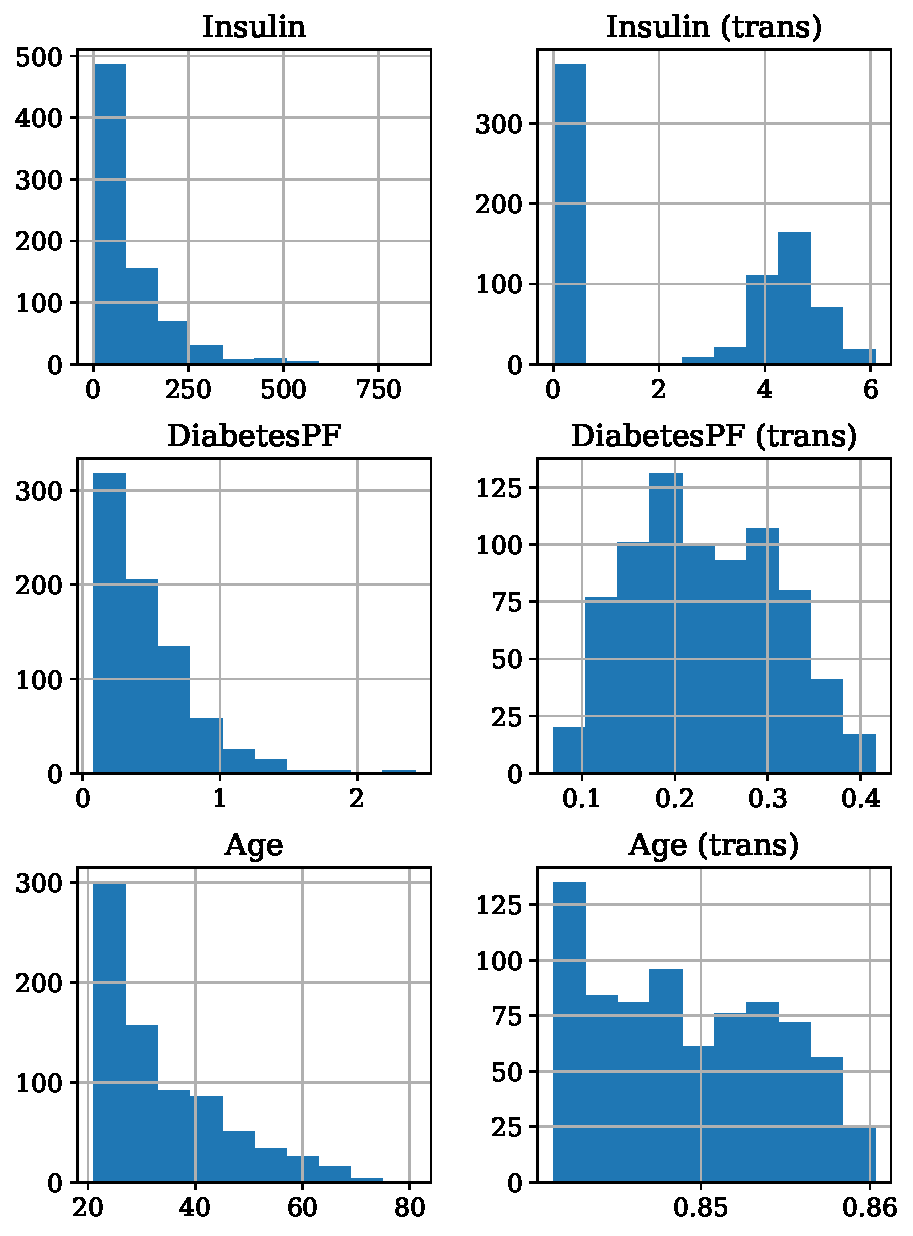
\includegraphics[width=0.5\textwidth]{figures/dist.pdf}
	\vspace{-0.7cm}
	\caption{The original and transformed distributions of the three most skewed features of the Pima Indians Diabetes Dataset}
	\label{skew_dist}
\end{figure}
\begin{figure}[!t]  % H
	\centering
	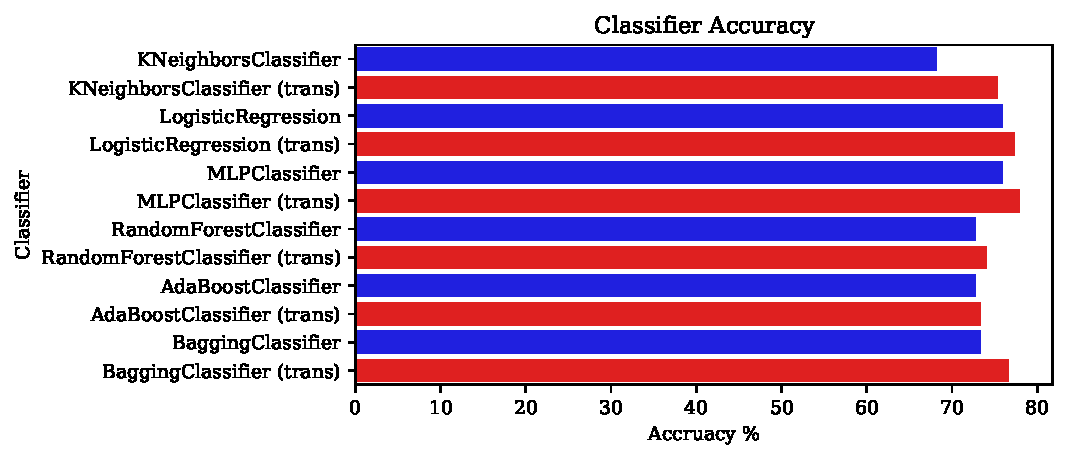
\includegraphics[width=0.5\textwidth]{figures/classifiers.pdf}
	\vspace{-0.7cm}
	\caption{The model accuracy of different classifiers based on the original (green bars) and transformed (red bars) distributions of the three most skewed features of the Pima Indians Diabetes Dataset}
	\label{skew_acc}
\end{figure}
The results show that the transformed feature distribution mitigates the skewness as one of the distributional properties of training data. We can see the accuracy improvement of all classifiers in the presence of transformed features. Therefore, the skewed training data features can negatively impact the DNN performance. This result also indicates the necessity of considering statistical and distributional properties of input data in initializing data opinions before propagation through the DNN network. 

\vspace {.2cm}
\noindent
\textbf{Second experiment.} Datasets used to train DNN models can be considerably different in terms of their statistical properties. Thus, we used the equally-weighted average of two distinct groups of statistical factors for each data opinion determinant (belief, disbelief, and uncertainty) for each dataset. We run the experiment for two group of factors: Cronbach's Alpha, Data Quality Score (DQS), and Eigenvalue ratio (explained variance) as the first group and Skewness, Kurtosis, and the Distributional Variance as the second group. We first run the experiment for each group of factors separately and then together. In Figures~\ref{susy_op} and~\ref{kdd_op}, there are two lines, blue and red, indicating the change in model opinion determinants as well as projected probability of the model considering first and second group of data opinion initialization factors, respectively. The green line also indicates the change in model opinion determinants and its projected probability considering both sets of factors simultaneously by the equally-weighted average. 

During training epochs, in Figures~\ref{susy_op} and~\ref{kdd_op}, we can see the increasing change in model belief as well as the decreasing change in model uncertainty for both datasets considering different factors separately and together. Therefore, each opinion determinant is relatively improved during training epochs.
Figures~\ref{susy_loss} and~\ref{kdd_loss} illustrate that the training process over datasets has been performed effectively for both datasets as decreasing loss and increasing accuracy during the training process shown in these figures is a sign of successful learning process. A successful training leads to the increase in model belief and projected probability as a measure of trustworthiness for both datasets while our model uncertainty is decreasing significantly. Thus, the projected probability is positively correlated with the model performance, and we can trust the DNN model much more than before after a successful training process. In comparison with the other trained models in case of similar accuracy, we can make a decision to select the model with higher projected probability at first, and in case of no significant discrepancy, the model with higher belief, lower disbelief, and lower uncertainty will be selected. In addition, we see a very low amount of disbelief and insignificant change (less than 0.01) in disbelief during training which is convincing since our input data that fed to the DNN were in high quality without missing or misleading data records. 

We report the average performance results as well as initial and ultimate model opinions during 5 distinct runs for each dataset in Table~\ref{result}. In this table, the model opinion determinants for training and testing phases over each dataset are updated and improved based on the loss function and accuracy achieved during a total number of training epochs. Note that the total belief of the model has been increased compared to the first epoch of training while the uncertainty has been relatively decreased. This result confirms the impact of successful training and loss optimization on the quantification and propagation of the total opinion's determinants. As the loss function is being minimized during training epochs, the accuracy of the entire network is increasing. Therefore, the model accuracy in training time is correlated to the belief and uncertainty of the model opinion. Since the opinion determinants have additivity requirement, change in one determinants coincides with changes in other determinants. 
%t and they vary with respect to each other based on Table~\ref{result}. 
We can also see the improvement in the trustworthiness or projected probability of the model while training is performed. Note the difference between the projected probability in total opinion (after training) compared to the first epoch of training such that the total projected probability of the model has been increased compared to the starting point of training. Note that we could achieve better performance by hyperparameter tuning and/or increasing the number of training epochs. However, this improvement was irrelevant to the objectives of the experiment.  
%impact on the objectives of the expriments  intent of the experiment was only to  to perform just a convincing and ordinary training and testing process. 



% In addition, any suitable value for each hyperparameter in our model like the number of required training epochs for convergence, the initial amount of learning rate, and the optimization approach can be leveraged to achieve the best possible accuracy.

\begin{figure*}[!ht]  % H
	\centering
	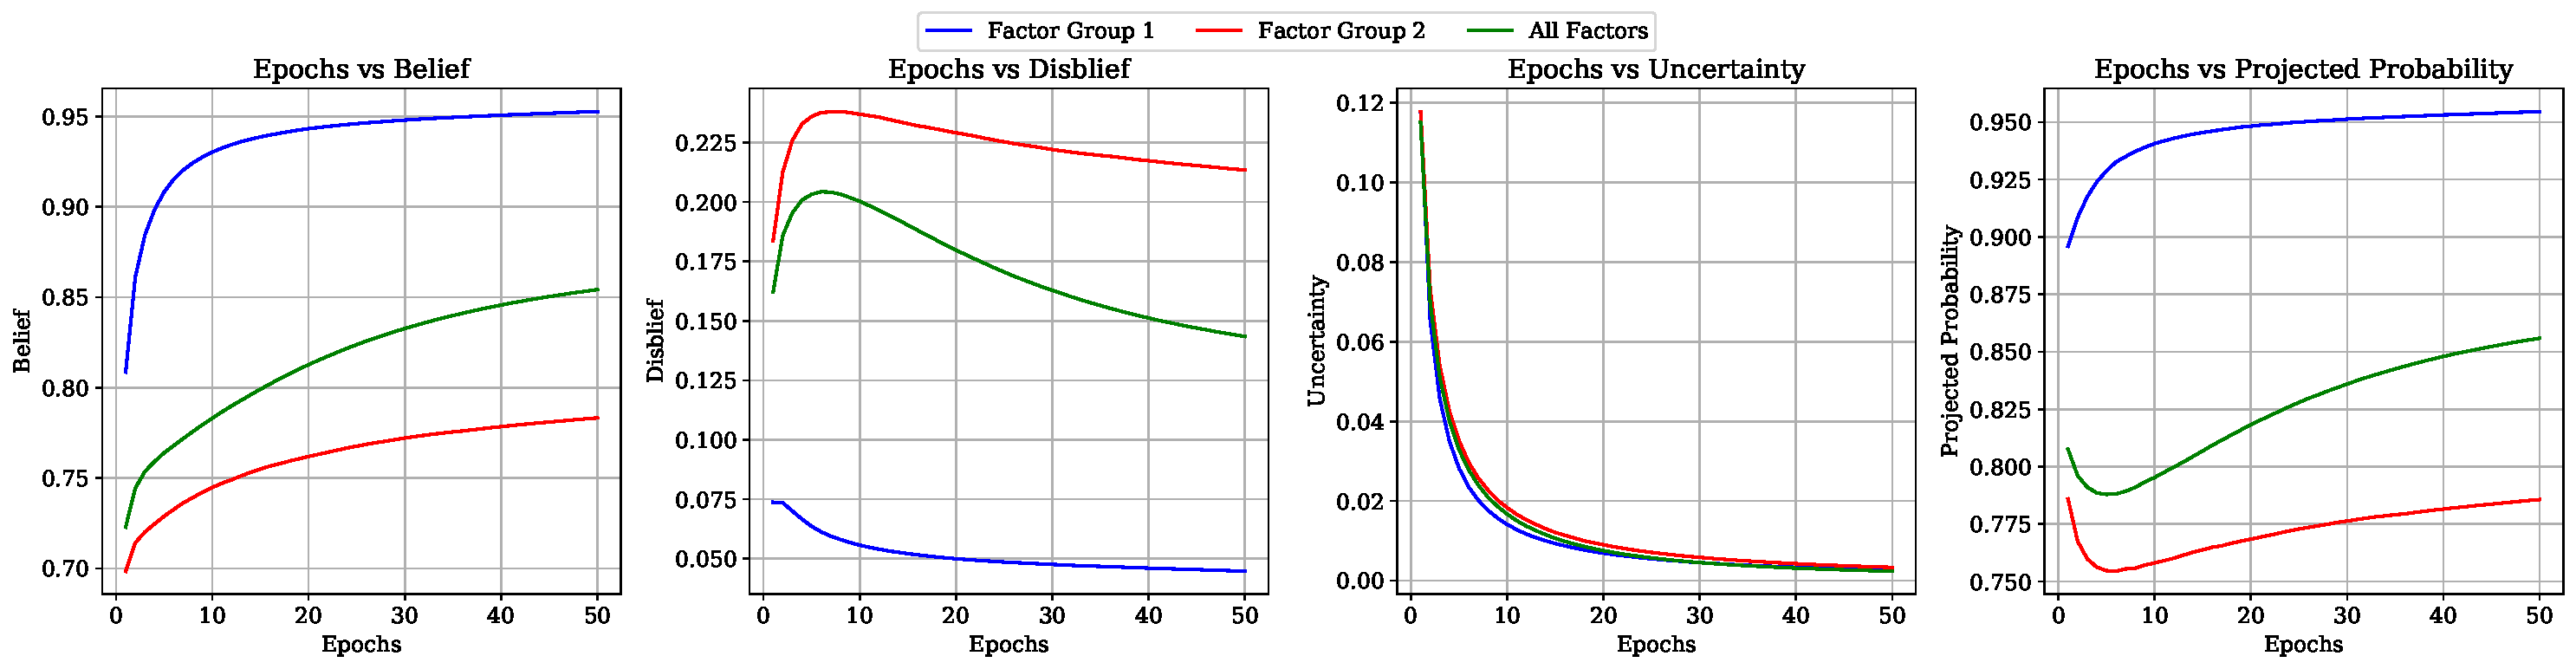
\includegraphics[scale=0.5, width=\textwidth]{figures/Results_Op_susy.pdf}
	\caption{The improvement process of opinion determinants during 45 training epochs based on different factors in numerical features over SUSY dataset}
	\label{susy_op}
\end{figure*}
\begin{figure*}[!ht]
	\centering
	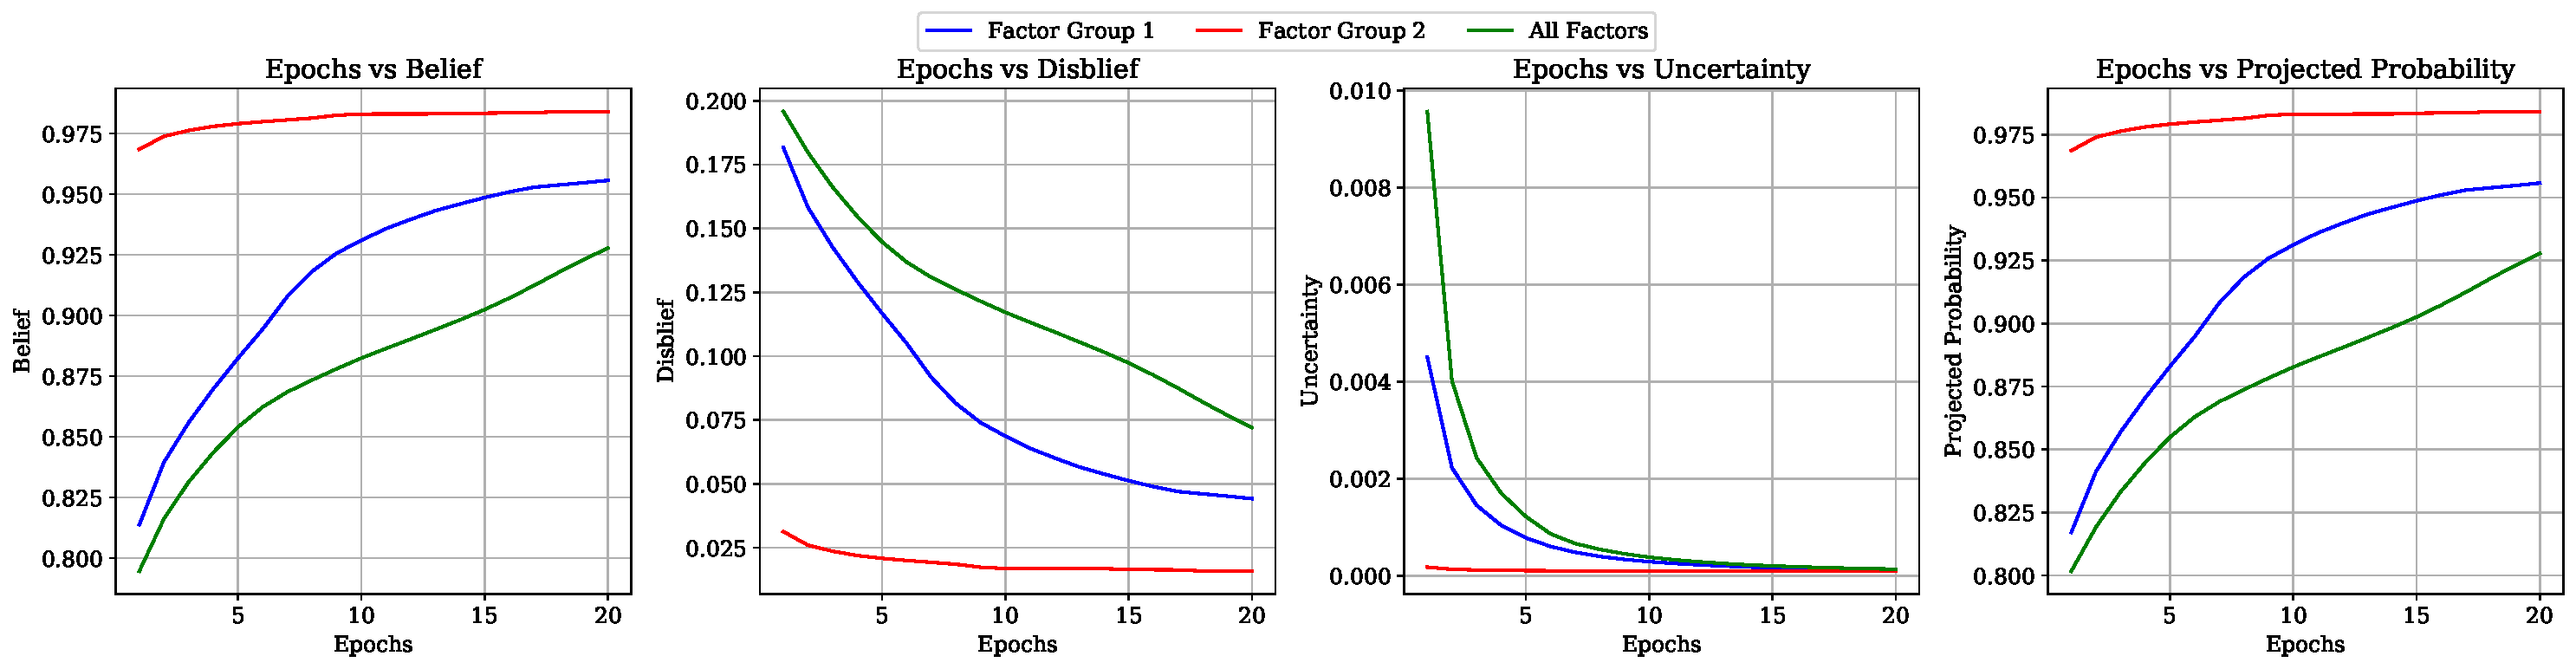
\includegraphics[scale=0.5, width=\textwidth]{figures/Results_Op_kdd.pdf}
	\caption{The improvement process of opinion determinants during 20 training epochs based on different factors in numerical features over KDD Cup 99 dataset}
	\label{kdd_op}
\end{figure*}
\begin{figure}[!ht]  % H
	\centering
	\includegraphics[width=0.5\textwidth]{figures/susy_res.pdf}
	\vspace{-0.7cm}
	\caption{The accuracy and loss values during 45 training epochs over SUSY dataset}
	\label{susy_loss}
\end{figure}
\begin{figure}[!ht] % H
\centering
\includegraphics[width=0.5\textwidth]{figures/kdd_res.pdf}
\vspace{-0.7cm}
\caption{The accuracy and loss values during 20 training epochs over KDD Cup 99 dataset}
\label{kdd_loss}
\end{figure}
\begin{table*}[!ht]
% \hskip -1.3cm
\centering
\begin{tabular}{c c cccc cccc}
    \toprule
\multirow{2}{*}{\textbf{Dataset}} 
        & \multicolumn{1}{c}{\textbf{Performance}} & \multicolumn{4}{c}{\textbf{1st Training Epoch Opinion}} &
        \multicolumn{4}{c}{\textbf{Total Opinion}} \\
    \cmidrule(lr){2-2} \cmidrule(lr){3-6} \cmidrule(lr){7-10}
        & Total Accuracy & Belief & Disbelief & Uncertainty & Proj. Prob. & Belief  & Disbelief & Uncertainty & Proj. Prob. \\
    \midrule
SUSY: \textit{Training} 
        & 72.863\%  & 0.6420 & 0.0160 & 0.3420 & 0.8130 & 0.8470 & 0.0080 & 0.1440 & 0.9640      \\
    \addlinespace
SUSY: \textit{Testing}
        & 69.785\%   & - & - & - & - &  0.8495 & 0.0089 & 0.1417 & 0.9203        \\
    \addlinespace
KDDCup99: \textit{Training}
        & 99.065\%  & 0.9280 & 0.0050 & 0.0670 & 0.9610 & 0.9978 & 0.0002 & 0.0021 & 0.9981 \\
    \addlinespace
KDDCup99: \textit{Testing}
        & 97.846\%   &  -   &  -  &  -  & - &  0.9969 & 0.0002 & 0.0029 & 0.9970    \\
    % \addlinespace

% \multirow{4}{*}{KDD Cup 99}
%         & item 1    & item 2    & then 3    & item 4    & item 5    & item 6            \\
%         & item 1    & item 2    & then 3    & item 4    & item 5    & item 6            \\
%         & item 1    & item 2    & then 3    & item 4    & item 5    & item 6            \\
%         & item 1    & item 2    & then 3    & item 4    & item 5    & item 6            \\
    \bottomrule
\end{tabular}
\vspace{2mm}
\caption{The average performance and opinion results for training and testing time during 5 different runs over each dataset}
\label{result}
\end{table*}
In conclusion, our evaluation demonstrates that the opinion quantification process is adequately flexible when statistical properties of the input data is incorporated in to the process. Note that the selection of these statistical factors can be different for one model to another based on the characteristics of the application domain. For example, in a medical domain the reliability of input data could be a major factor in opinion generation while in another domain the skewness or kurtosis of data can have higher priority to be considered.

%Another advantage of incorporating statestical poroperties of input data in opinion propagation is its contribution to the interperqatbility and explainability of the  is the 


%charactristicsstatistical properties of the input dataset. These independent factors for data opinion initialization should be explainable and interpretable based on the nature of feature distributions, the task objective, and the application domain. We can also apply different weights for different factors in the proposed approach to tune the impact of each factor in initializing data opinion determinants. 

%the proposed data opinion propagation approach is adequately flexible for different DNN architectures.

%since based on the nature of input data and its features, any appropriate architecture of neural network can be utilized to train the model and achieve the best possible performance. 

%initialization approach for data feature opinions is constructed based on statistical properties of input data, also comprehensively flexible. Everyone can exploit and add more different and independent statistical factors, combined by weighted average, to initialize the data opinion determinants, even for the categorical features' opinions as well. 















% Confusion matrices in the Figure~\ref{susy_cm} and~\ref{kdd_cm} demonstrate that the trained model could achieve good results and acceptable accuracy over unseen data (test data).

% \begin{figure}[H]
% 	\centering
% 	\includegraphics[scale=0.5]{figures/susy_cm.PNG}
% 	\caption{A Confusion matrix for testing over SUSY dataset}
% 	\label{susy_cm}
% \end{figure}
% \begin{figure}[H]
% 	\centering
% 	\includegraphics[scale=0.5]{figures/kdd_cm.PNG}
% 	\caption{A Confusion matrix for testing over KDD Cup 99 dataset}
% 	\label{kdd_cm}
% \end{figure}


%%%%%%%%%%%%%%%%%%%%%%%%%%%%%%%%%%%%%%%%%%%%%%%%%%%%%%%%%%%%%%%

% \usepackage{booktabs, multirow}


% \begin{table}
% \centering
% \begin{tabular}{c ccc ccc}
%     \toprule
% \multirow{2}{*}{two rows} 
%         & \multicolumn{3}{c}{3-columns cell} & \multicolumn{3}{c}{3-columns cell}   \\
%     \cmidrule(lr){2-4} \cmidrule(lr){5-7}
%         & column 1  & column 2  & column 3  & column 4  & column 5  & column 6          \\
%     \midrule
% \multirow{4}{*}{Social Network}  
%         & item 1    & item 2    & then 3    & item 4    & item 5    & item 6            \\
%         & item 1    & item 2    & then 3    & item 4    & item 5    & item 6            \\
%         & item 1    & item 2    & then 3    & item 4    & item 5    & item 6            \\
%         & item 1    & item 2    & then 3    & item 4    & item 5    & item 6            \\
%     \addlinespace
% \multirow{4}{*}{Citation Dataset}
%         & item 1    & item 2    & then 3    & item 4    & item 5    & item 6            \\
%         & item 1    & item 2    & then 3    & item 4    & item 5    & item 6            \\
%         & item 1    & item 2    & then 3    & item 4    & item 5    & item 6            \\
%         & item 1    & item 2    & then 3    & item 4    & item 5    & item 6            \\
% \bottomrule
% \end{tabular}
% \caption{Example of professional table design}
%     \end{table}


% \begin{table}[t]
% \begin{tabular*}{\columnwidth}{@{\extracolsep{\fill}}%
%     l T{4}T{2}T{2}T{4}}
% \toprule
% Year & {Nones}& {Option 1} & {Option 2} & {Total} \\
% \midrule
%   2001& 126   & 16    & 2     & 144 \\
%   2002& 114   & 9     & 4     & 127 \\
%   2003& 115   & 7     & 1     & 123 \\
%   2004& 114   & 6     & 4     & 124 \\
%   2005& 104   & 5     & 8     & 117 \\
%   2006& 96    & 3     & 6     & 105 \\
%   2007& 93    & 2     & 4     & 99 \\
%   2008& 93    & 2     & 2     & 97 \\
%   2009& 85    & 2     & 11    & 98 \\
%   2010& 83    & 0     & 7     & 90 \\
%   2011& 74    & 0     & 12    & 86 \\
%   \midrule
%   Total & 1097 & 52   & 61    & 1210 \\
% \bottomrule
% \end{tabular*}
% \end{table}



% \begin{table*}
% %
% \tablestyle[sansbold]
% %
% \begin{tabular}{*{2}{p{0.45\textwidth}}}
% \theadstart
%     \thead header &
%     \thead header \\
% \tbody
%  %
%  content  & content \\
%  content  & content \\
%  content  & content \\
%  %
%  \tsubheadstart
%  \tsubhead subhead &
%  \tsubhead subhead \\
%  %
%  content  & content \\
%  content  & content \\
%  \tend
% \end{tabular}
% \vspace{2mm}
% \caption{sansbold style}
% \label{tab:style:sansbold}
% \end{table*} 